\documentclass{standalone}
\usepackage{tikz}
\usepackage{ctex,siunitx}
\setCJKmainfont{Noto Serif CJK SC}
\usepackage{tkz-euclide}
\usepackage{amsmath}
\usetikzlibrary{patterns, calc,3d}
\usetikzlibrary {decorations.pathmorphing,decorations.pathreplacing,decorations.shapes}
\begin{document}
\small
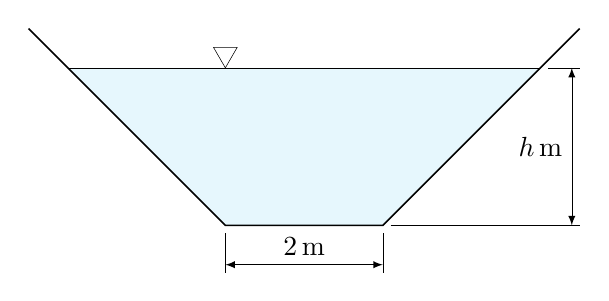
\begin{tikzpicture}[>=latex,scale=1.0]
  \fill[cyan!10!white](-3,2)--(-1,0)--(1,0)--(3,2);
  \draw[semithick](-3.5,2.5)--(-1,0)--(1,0)--(3.5,2.5);
  \draw[very thin](-3,2)--(3,2);
  \draw[very thin](-1,2)--++(60:0.3)--++(180:0.3)--++(-60:0.3);
  \draw[very thin](-1,-0.1)--++(0,-0.5)(1,-0.1)--++(0,-0.5)(1.1,0)--(3.5,0)(3.1,2)--(3.5,2);
  \draw[very thin,<->](-1,-0.5)--(1,-0.5)node[midway,above]{\qty{2}{m}};
  \draw[very thin,<->](3.4,0)--(3.4,2)node[midway,left]{$h$\,\unit{m}};
\end{tikzpicture}
\end{document}